The literature review is about 60\%, though further reading might prove that 
this number might change. Our objective this year is to generate a 
video-to-spike train encoder. For this, the first approach was to use a
biologically plausible functional model \cite{basab-model} that results in
images being transformed into rank-ordered spikes 
\cite{thorpe-spike-rapid-processing}.

\begin{figure}[hbt]
  \centering
  \begin{subfigure}[b]{0.15\textwidth}
    \centering
    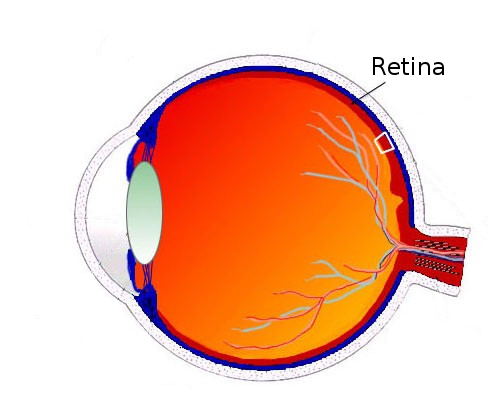
\includegraphics[width=\textwidth,valign=t]{Sagschem}
    \caption{Eye schematics}
    \label{sub-fig-eye-schematics}
  \end{subfigure}
  \begin{subfigure}[b]{0.15\textwidth}
    \centering
    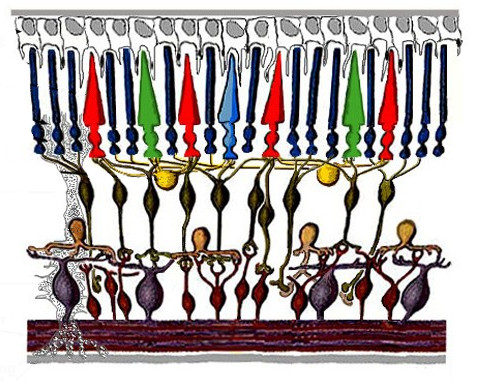
\includegraphics[width=\textwidth,valign=t]{schem}
    \caption{Retina}
    \label{sub-fig-retinal-layers}
  \end{subfigure}
  \begin{subfigure}[b]{0.15\textwidth}
    \centering
    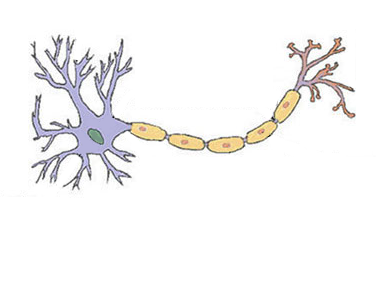
\includegraphics[width=\textwidth,valign=t]{Neuron-___-wikimedia-org}
    \caption{Neuron}
    \label{sub-fig-neuron}
  \end{subfigure}
  
  \caption{Anatomy of the (human) eye }
  \label{fig-basic-eye-anatomy}
\end{figure}

The retina is a thin layer of neural cells located in the eye (Fig. 
\ref{fig-basic-eye-anatomy}), it is responsible
for the sensing, processing and transmitting visual input\cite{webvision}. 
At its deepest layer, the retina has a millions of cells known as 
photoreceptors (top of Fig. \ref{sub-fig-retinal-layers}), they are in charge 
of transforming light into electrical 
signals. After this step there are, mainly, three layers of neurons that 
perform different computations such as lateral inhibition or on/off 
centre-off/on surround behaviour\cite{webvision, basab-model}. A small area 
at the centre of the retina has very few obstacles to obtain light and has high
resolution, this area is known as the \emph{foveal pit} (small depression on 
the right of Fig. \ref{sub-fig-eye-schematics}).

\begin{figure}[hbt]
  \centering
  \begin{subfigure}[t]{0.15\textwidth}
    \centering
    \captionsetup{justification=centering,margin=0.1cm}
    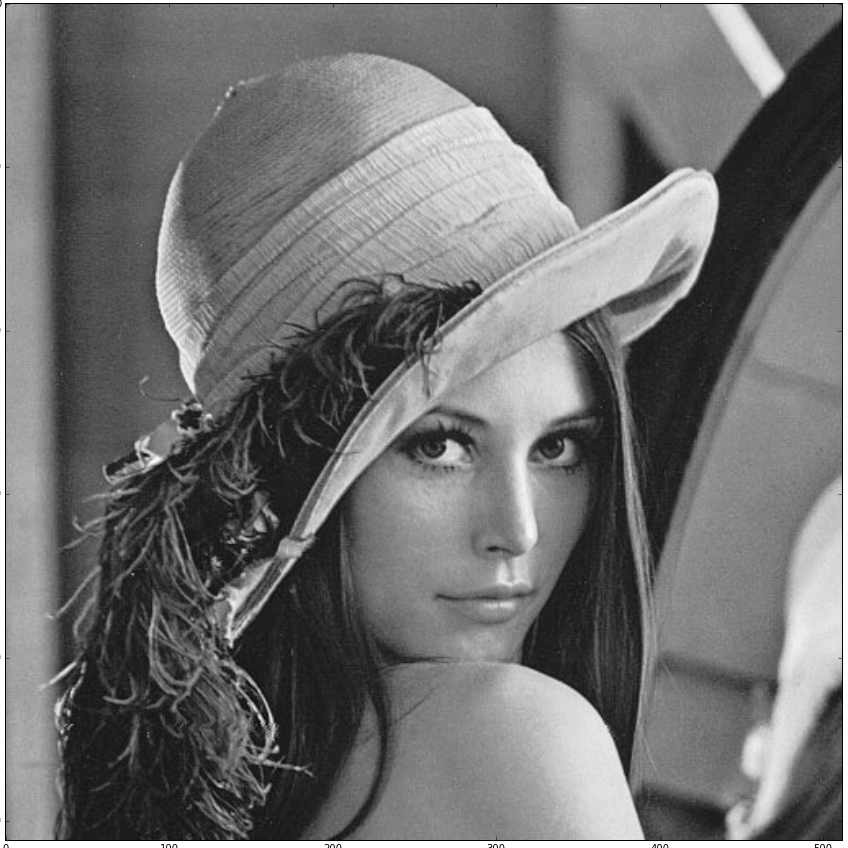
\includegraphics[width=\textwidth]{./Lena-gray}
    \caption{Original image}
    \label{pic-lena}
  \end{subfigure}
  \begin{subfigure}[t]{0.15\textwidth}
    \centering
    \captionsetup{justification=centering,margin=0.1cm}
    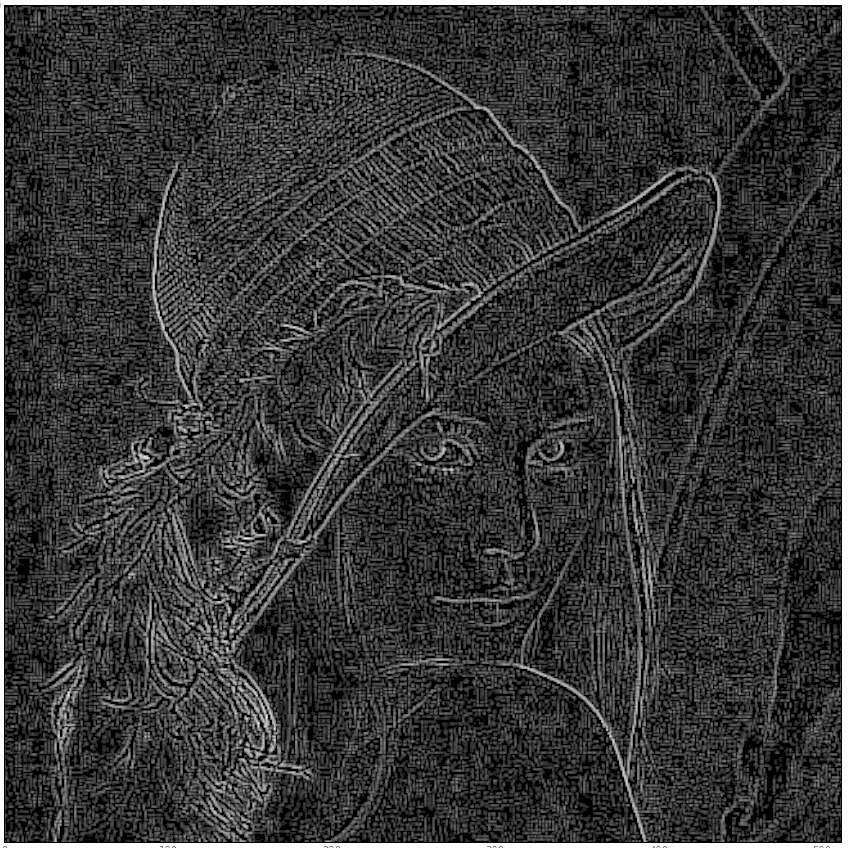
\includegraphics[width=\textwidth]{./Lena-midget_off}
    \caption{Midget OFF-centre}
    \label{pic-lena-M-OFF}
  \end{subfigure}
  \begin{subfigure}[t]{0.15\textwidth}
    \centering
    \captionsetup{justification=centering,margin=0.1cm}
    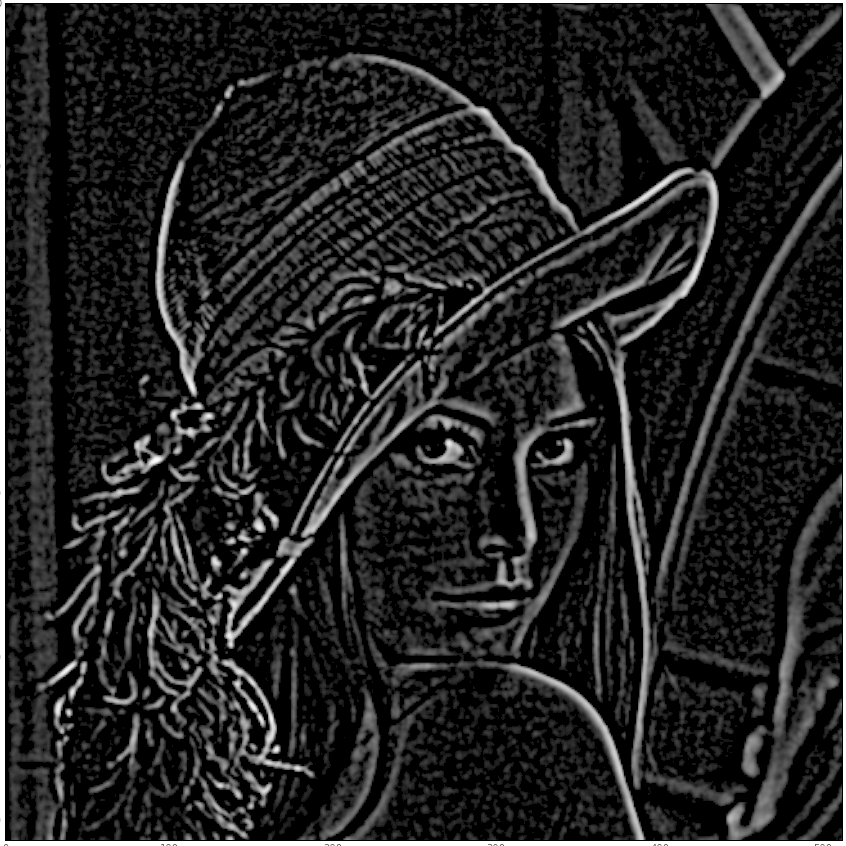
\includegraphics[width=\textwidth]{./Lena-midget_on}
    \caption{Midget ON-centre}
    \label{pic-lena-M-ON}
  \end{subfigure}
  \begin{subfigure}[t]{0.15\textwidth}
    \centering
    \captionsetup{justification=centering,margin=0.1cm}
    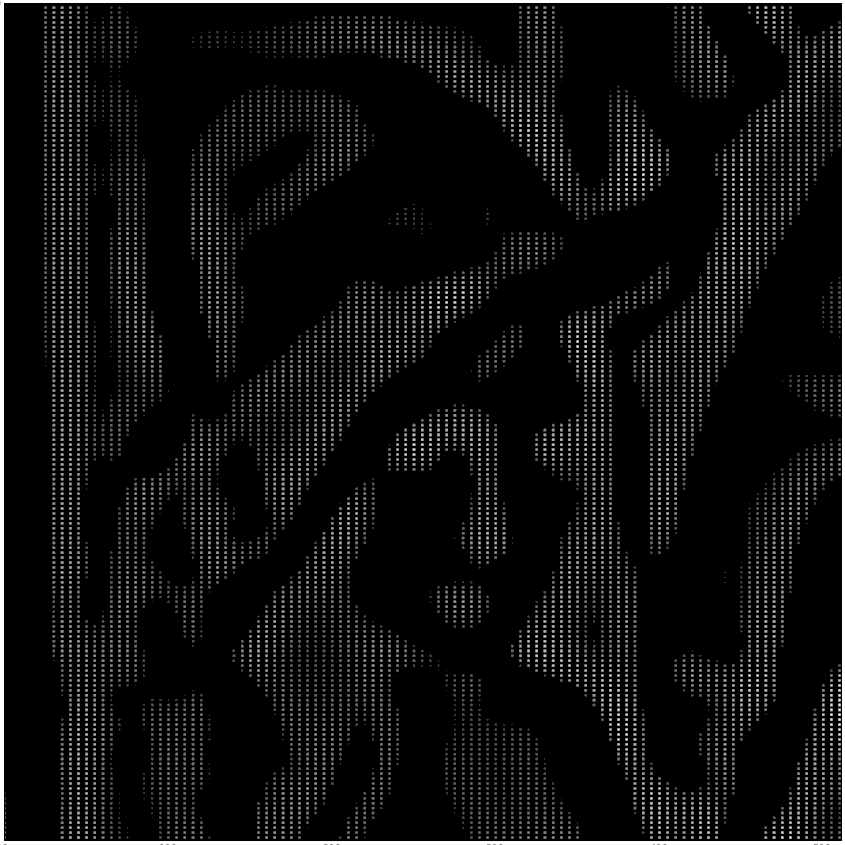
\includegraphics[width=\textwidth]{./Lena-parasol_off}
    \caption{Parasol OFF-centre}
    \label{pic-lena-P-OFF}
  \end{subfigure}
  \begin{subfigure}[t]{0.15\textwidth}
    \centering
    \captionsetup{justification=centering,margin=0.1cm}
    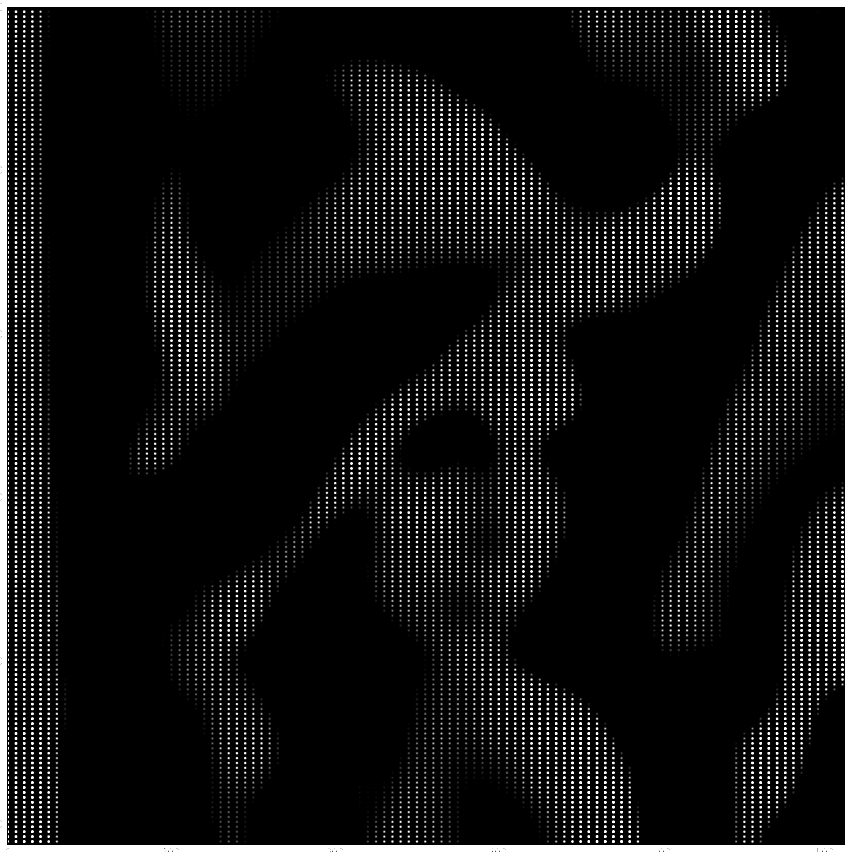
\includegraphics[width=\textwidth]{./Lena-parasol_on}
    \caption{Parasol ON-centre}
    \label{pic-lena-P-ON}
  \end{subfigure}
  \caption{Results of simulating ganglion cells (convoluted images are enhanced for better contrast)}
  \label{fig-convolution-results}
\end{figure}
This algorithm models the foveal pit, first we perform a two-dimensional  
\emph{convolution} of the current frame with four different \emph{kernels}
which represent four types of ganglion cells (Fig. 
\ref{fig-convolution-results}). Each pixel in the convoluted images represent a 
spike emission time, the higher the pixel value, the sooner the spike will be 
sent out. Convolution alone is a compute intensive task and we obtain about 12
frames-per-second (FPS) on a Core i5-4570 CPU @ 3.20GHz with 8 GBytes of 64-bit 
DDR3 RAM @ 1600MHz and a GeForce GT 720 GPU with 192 CUDA cores, 1GBytes of 64-bit DDR3 RAM.
.
\begin{table}[hbt]
  \begin{center}
    \caption{Performance comparison.}
    \bgroup
    \def\arraystretch{1.2}
    \begin{tabular}{l c c c c}
%      \begin{minipage}{1.2cm} \vspace*{0.2cm}Algorithm \vspace*{0.001cm}\end{minipage}& 
      &
      \begin{minipage}{1.2cm}Midget Off-centre\vspace*{0.05cm}\end{minipage} & 
      \begin{minipage}{1.2cm}Midget On-centre\vspace*{0.05cm}\end{minipage}& 
      \begin{minipage}{1.2cm}Parasol Off-centre\vspace*{0.05cm}\end{minipage}& 
      \begin{minipage}{1.2cm}Parasol On-centre\vspace*{0.05cm}\end{minipage}\\
      \hline 
      Naïve     & 0.0009s & 0.0031s & 0.0587s & N/A\footnote{Unable to fit convolution kernel into constant memory.} \\ 
      Separated & 0.0029s & 0.0055s & 0.0172s & 0.0472s \\ 
      Tiled     & 0.0019s & 0.0027s & N/A\footnote{ Coding optimizations are still in progress.} & N/A$^2$ \\ 
       
    \end{tabular} 
    \egroup
  \end{center}
\end{table}
\vspace*{-10pt}

In the retina, redundancy of information is reduced via lateral inhibition 
prior to any ganglion cell activity. In this algorithm, we perform a correction 
is on the convolved images by adjusting the convoluted image's weights 
according to the correlation between convolution kernels. The results of using
correction or not can be appreciated on Fig. \ref{fig-reconstruction}; 
furthermore using only 30\% of the corrected weight, enough visual information 
is transmitted\cite{basab-model}.

\begin{figure}[hbt]
  \centering
  \begin{subfigure}[t]{0.15\textwidth}
    \centering
    \captionsetup{justification=centering,margin=0.1cm}
    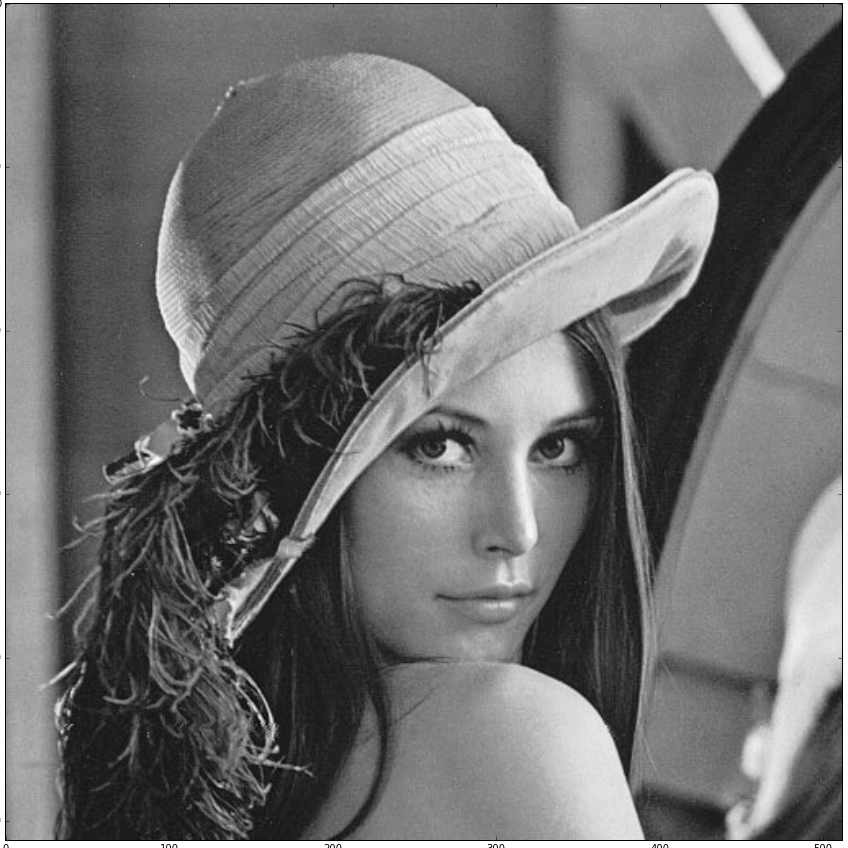
\includegraphics[width=\textwidth]{./Lena-gray}
    \caption{Original image}
    \label{pic-original-lena}
  \end{subfigure}
  \begin{subfigure}[t]{0.15\textwidth}
    \centering
    \captionsetup{justification=centering,margin=0.1cm}
    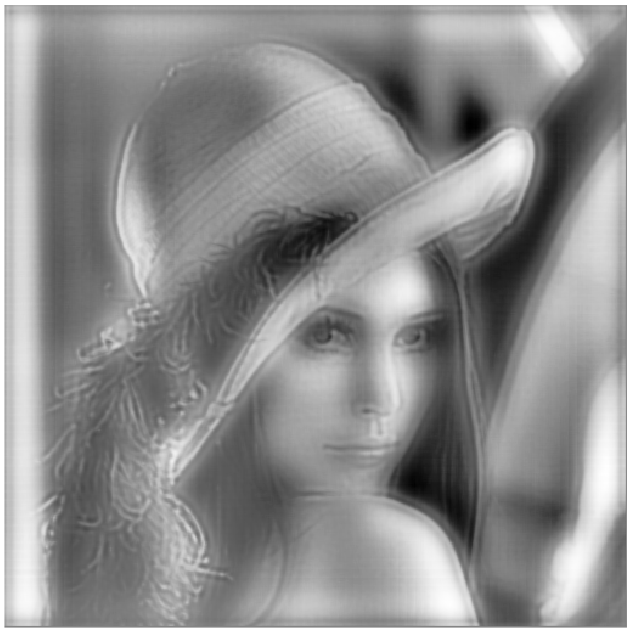
\includegraphics[width=\textwidth]{./final_results-unfiltered}
    \caption{100\% raw spikes}
    \label{pic-unfiltered-spikes}
  \end{subfigure}
  %        \hfill
  \begin{subfigure}[t]{0.15\textwidth}
    \centering
    \captionsetup{justification=centering,margin=0.1cm}
    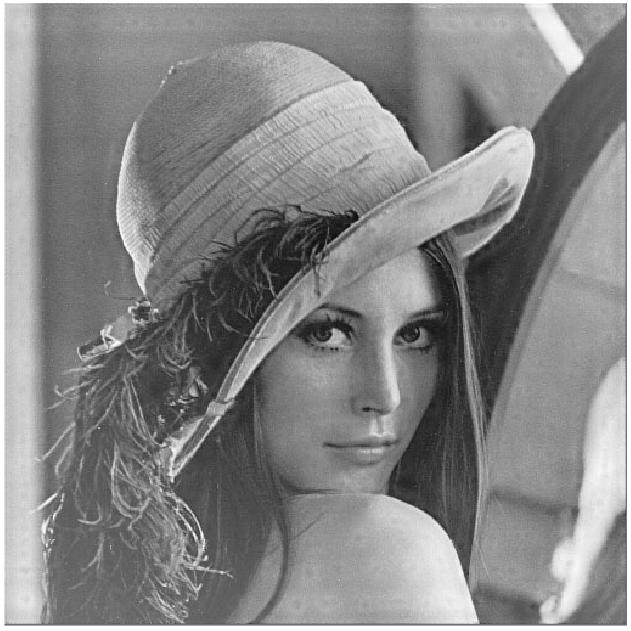
\includegraphics[width=\textwidth]{./final_results-focal-100}
    \caption{100\% \emph{corrected} spikes}
    \label{pic-100pc-spikes}
  \end{subfigure}
%  \begin{subfigure}[t]{0.15\textwidth}
%    \centering
%    \captionsetup{justification=centering,margin=0.1cm}
%    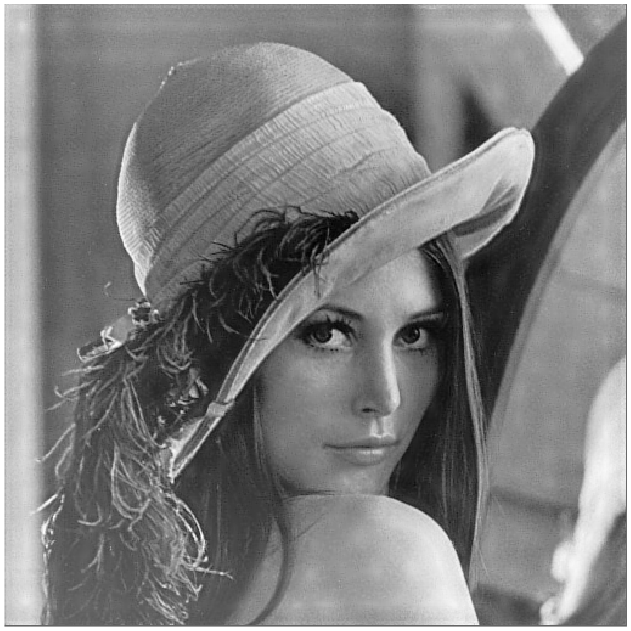
\includegraphics[width=\textwidth]{./final_results-focal-30pc}
%    \caption{\\30\% of \emph{corrected} spikes}
%    \label{pic-30pc-spikes}
%  \end{subfigure}
  \caption{Results of reconstruction procedure}
  \label{fig-reconstruction}
\end{figure}
Correcting the spikes for redundancy is a highly consuming task which might be 
better suited for event-based programming, such as the one found on the 
SpiNNaker platform. We are still working on an implementation for this 
approach.

A second way of encoding is to simulate the early stages of the retina, which
sense changes in intensity on the photoreceptors. This is quite similar to what 
DVS do \cite{aer-retina-bernabe, dvs-zurich}, but with limited dynamic range 
and lower temporal resolution. The main advantage is that no specialized 
hardware is needed and the operation is so fast that any recent computer should
be able to do it. For this type of encoding procedure we hypothesize that
the bigger the change, the sooner a cell would spike and, thus, we can obtain
a spike timings given the difference of two video frames. This project is also
on its final stages, though more testing is required.

